\chapter{Ανιχνευτικό Σύστημα }

	Όπως έχουμε ήδη αναφέρει ο RHIC επιταχύνει αντίθετα περιστρεφόμενες δέσμες βαρέων ιόντων, πρωτονίων και πρωτονίων με πολωμένο σπιν εως 50-60\% με στόχο να τις συγκρούει σε 6 διαφορετικά σημεία. Στα τέσσερα από αυτά υπήρχαν, από την αρχή της λειτουργίας του, ανιχνευτές οι οποίοι ήταν σχεδιασμένοι έτσι ώστε ο καθένας να μελετά διαφορετικά χαρακτηριστικά των συγκρούσεων.
	
	 Οι δύο πιό μικροί, ο PHOBOS και ο BRAHMS είναι πλέον εκτός λειτουργίας. Ο PHOBOS ήταν σχεδιασμένος ώστε να μελετάει τις συγκρούσεις ιόντων χρυσού αναλύοντας μόλις το 1\% των συνολικών γεγονότων. Κατά την λειτουργία του παρείχε μετρήσεις για την θερμοκρασία, το μέγεθος του αποτελέσματος του κάθε γεγονότος , καθώς και την αναλογία των διάφορων τελικών σωματιδίων με σκοπό τον προσδιορισμό της μετάβασης φάσης μεταξύ της συνήθους ύλης και του QGP (Quark Gluon Plasma). Ο BRAHMS στόχευε στην μελέτη των φορτισμένων αδρονίων για μεγάλο έυρος τιμών pseudo-rapidity και ορμής κάθετης στην δέσμη (Transverse Momentum $p_T$), προκειμένου να γίνει κατανοητός ο μηχανισμός συμπεριφοράς της διεγερμένης πυρηνικής ύλης που δημιουργείται κατά τις συγκρούσεις. 
	
	Ο πιό μεγάλος ανιχνευτής, ο PHENIX, έχει σταματήσει την λειτουργία του από το 2016 και τώρα αναβαθμίζεται στον sPHENIX. Αυτός στόχευε στην ανίχνευση των φωτονίων και των λεπτονίων, τα οποία δεν αλληλεπιδρούν μέσω της ισχυρής πυρηνικής αλληλεπίδρασης και γι' αυτό σε αυτά υπάρχουν πληροφορίες προερχόμενες απευθείας από τις αρχικές συγκρούσεις των ιόντων. 
	
	Τέλος, ο ανιχνευτής STAR (Solenoidal Tracker) είναι ο μόνος που λειτουργεί ακόμη (Εικόνα (\ref{im3.1}). Ο κυριότερος από τους αρχικούς στόχους του STAR %\textcolor{green}{[Overview of STAR Detector]} 
	ήταν να μελετήσει την ισχυρά αλληλεπιδρώσα ύλη σε υψηλή πυκνότητα ενέργειας και αναλύοντας ταυτόχρονα πολλά γεγονότα, να βρει ενδείξεις για την πιθανή δημιουργία αλλά και την χωροχρονική εξέλιξη του QGP που δημιουργείται υπό αυτές τις συνθήκες υψηλής πυκνότητας ενέργειας και θερμοκρασίας. 
	Ακόμη, πρωταρχικός του στόχος είναι να μετρήσει την δομή του σπιν του πρωτονίου και την συνεισφορά των σπιν των γλουονίων σε αυτό, καθώς από πειράματα της εποχής υπήρχαν ενδείξεις ότι τα κουαρκ και τα αντικουαρκ συνεισφέρουν μόνο κατα $\sim25\%$. Αν κάτι τέτοιο ισχύει, τότε ο μόνος τρόπος εξήγησης του συνολικού σπιν του πρωτονίου θα ήταν μέσω της σχετικής κίνησης των κουάρκ-γλουονίων. Ακόμη, από τις συγκρούσεις πολωμένων πρωτονίων με $\sqrt{S}=500GeV$ από τις οποίοες παράγονται $W^{pm}$ στόχευαν στον προσδιορισμό της εξάρτησης της πόλωσης των αντικουάρκ από την γεύση.
	\begin{figure}[h!]
		\centering
		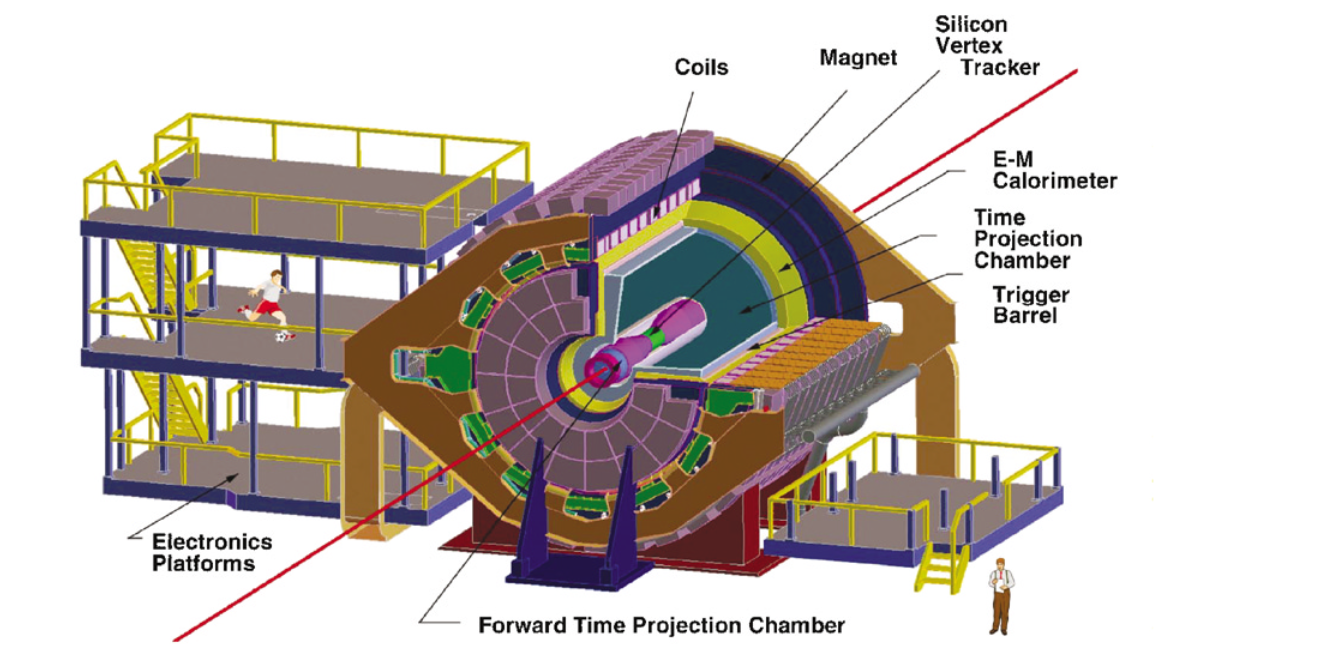
\includegraphics[scale=0.5]{STAR_Detectors/Star_Layout.png}
		\caption{Η δομή του STAR}
		\label{im3.1}
	\end{figure}
	
	Τέλος, στόχος ήταν να μελετήσει γεγονότα ultra-peripheral συγκρούσεων (UPC). Όταν η παράμετρος κρούσης είναι μεγαλύτερη από το άθροισμα των ακτινών των πυρήνων ή των πυρήνων-πρωτονίων ($b>R_1+R_2$), τότε οι ισχυρές αλληλεπιδράσεις είναι αδύνατες με αποτέλεσμα να έχουμε αλληλεπιδρλασεος μέσω συγκρούσεων φωτονίων-ιόντων και φωτονίων-φωτονίων. Τα φωτόνια εκπέμπονται από την κίνηση των σωματιδίων και η ροή τους είναι ανάλογη της τετραγωνικής ρίζας του φορτίου, άρα τα βαρέα ιόντα του RHIC είναι κατάλληλα για την μελέτη αυτών των αλλληλεπιδράσεων. 	
	
	
	Ο αριχκός σχεδιασμός του STAR περιλάμβανε έναν Silicon Vertex Tracker (SVT), κοντά στην περιοχή αλληλεπίδρασης, με 216 ανιχνευτές πυριτίου διαρυθμισμένους σε τρια κυλινδρικά στρώματα. Στην συνέχεια υπάρχει ένας Forward Time Projection Chamber (FTPC), ένας Time Projection Chamber (TPC) μεγάλου όγκου για ανίχνευση τροχιών και ταυτοποίηση των σωματιδίων , οποίος είναι και το μεγάλο πλεονέκτημα του STAR καθώς είναι κατάλληλος για την ανίχνευση των διαφορετικών προϊόντων των συγκρούσεων βαρέων ιόντων. Μετά υπάρχει ο Time of Flight ανιχνευτής και τα Ηλεκτρομαγνητικά Καλορίμετρα (Electromagnetic Calorimeter-EMC \& Endcap Electromagnetic Calorimeter-EEMC). Όλα αυτά είναι εντός ενός σωληνοειδούς που παράγει ισχυρό μαγνητικό πεδίο. Aκόμη, υπάρχει ένας Ring Imaging Cherenkov  Detector (RICH), για την ταυτοποίηση σωματιδίων με μεγαλύτερες κάθετες ορμές ($p_t$).% και στο εξωτερικό υπάρχει ένα Muon Telescope Detector (MTD) για την ανίχνευση μιονίων και την μέτρηση την ενέργειάς τους.
	
	Όλα τα παραπάνω, καθώς και άλλα συστήματα που δεν έχουν αναφερθεί, καταλαμβάνουν χώρο όσο ένα διόροφο κτίριο και ζυγίζουν πάνω από 1200 τόνους.
	Στην συνέχεια θα εξετάσουμε τους ανιχνευτές του STAR με μεγαλύτερη ακρίβεια. Κάποια από τα συστήματα που θα περιγραφούν δεν είναι πλέον σε λειτουργία και προφανώς ήταν αδύνατη η περιφραφή όλων των συστημάτων του STAR γι'αυτό και πολλά έχουν παραληφθεί.
	
	\begin{figure}[h!]
		\centering
		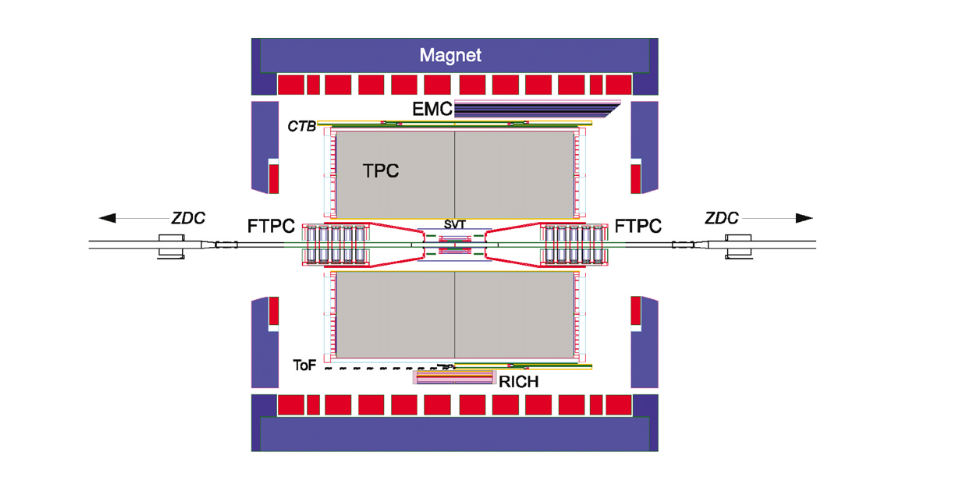
\includegraphics[scale=0.6]{STAR_Detectors/Cutway_Star_2001}
		\caption{Πλάγια τομή του STAR}
		\label{fig3}
	\end{figure}